\chapter{Modeling Lasing Threshold} \label{LT}


\section{History of Semiconductor Lasers} \label{corrections} As we know,
semiconductor lasers are important optoelectric devices ofr optical
communication systems. They are essential components for building optical
communication systems. There are intensive research results and achievements
from beginning.  In 1917, Einstein predicted the existence of spontaneous and
stimulated emission by which an atom can emit radiation. The first
semiconductor lasers were fabricated in 1962 using homojuncations. These lasers
had high threshold current density ( 19000/A/cm2 ) and operated at cryogenic
temperatures.  The concept of heterojuntion semiconductor lasers was realized
in 1969~1970 with a low threshold current density (1600 A/cm2) operating at
room temperature. These double-heterostructure diode lasers provide both
carrier and optical confinements, which imporve the efficiency for stimulated
emission.  The concept of quantum well structures for semicondcutor lasers was
proposed and realized experimentally in the late 1970s. The threshold current
density was reduced to about 500 A/cm, which improved the laser performance
significantly.

\section{Principle of Semiconductor Lasers} \label{corrections}

As we know, the semiconductor laser (or laser diode) in its simplest form is a
p-n junction of a single crystal of semiconductor material arranged in a
cavity, as shown in . The type and configuration of the material used to
determine the optical characteristics of the laser diode emission. Like others
in various oscillators or wave sources, the fundamental elements in the
semiconductor lasers are the following three elements: semiconductor band
structure (population inversion to provide gain mechanism), current injection
and P-N junction ( external pumping to make gain sustainable) and reflector of
cavity (feedback to provide coherence). The most common semiconductor lasers
are including Fabry-Perot(FP) or distributed feedback (DFB)/distributed Bragg
reflector (DBR) 

\subsection{Absorption of Light}

The light and matter interaction includes absorption, spontaneous emission and
stimulated emission, we first discuss the absorption of light by introducing
the absorption coeffiecient. This is the absorption rate without considering
the occupation factors.

Based on the following equations for different dimensionality.


\begin{equation}
\begin{aligned}
    \alpha_{3D}(\hbar\omega)= & C_0{|\hat{e}\cdot\bf{p}_{cv}|^2}(f_v-f_c)\\
    & \frac{1}{2\pi^2}(\frac{2m_r^\ast}{\hbar^2})^{3/_2}(\hbar\omega-E_g)^{1/_2},\\
    & C_0=\frac{\pi{e^2}}{n_r\epsilon_0{c}{m_0^2}\omega},
\end{aligned}
\label{eq:two}
\end{equation}

\begin{eqnarray}
\begin{aligned}
& \alpha_{2D}(\hbar\omega)=C_0{|\hat{e}\cdot\bf{p}_{cv}|^2}\frac{m_r^\ast}{\pi\hbar^2{L_z}},
\\
& \alpha_{1D}(\hbar\omega)=C_0{|\hat{e}\cdot\bf{p}_{cv}|^2}\frac{{(m_r^\ast)}^{3/_2}}{\pi\hbar{m_e^\ast}{L_x}{L_y}}\frac{1}{\sqrt{(\hbar\omega-E_g)}},
\end{aligned}
\label{eq:five}
\end{eqnarray}

The split plots of absorption coefficient for different dimensionality as in
Fig.~\ref{absrate_split}. Noted the unique shapes of density of states.

\begin{figure}
  \caption{Absorption Coefficient versus Photon Energy for 1D 2D and 3D with split plot}
  \centering
  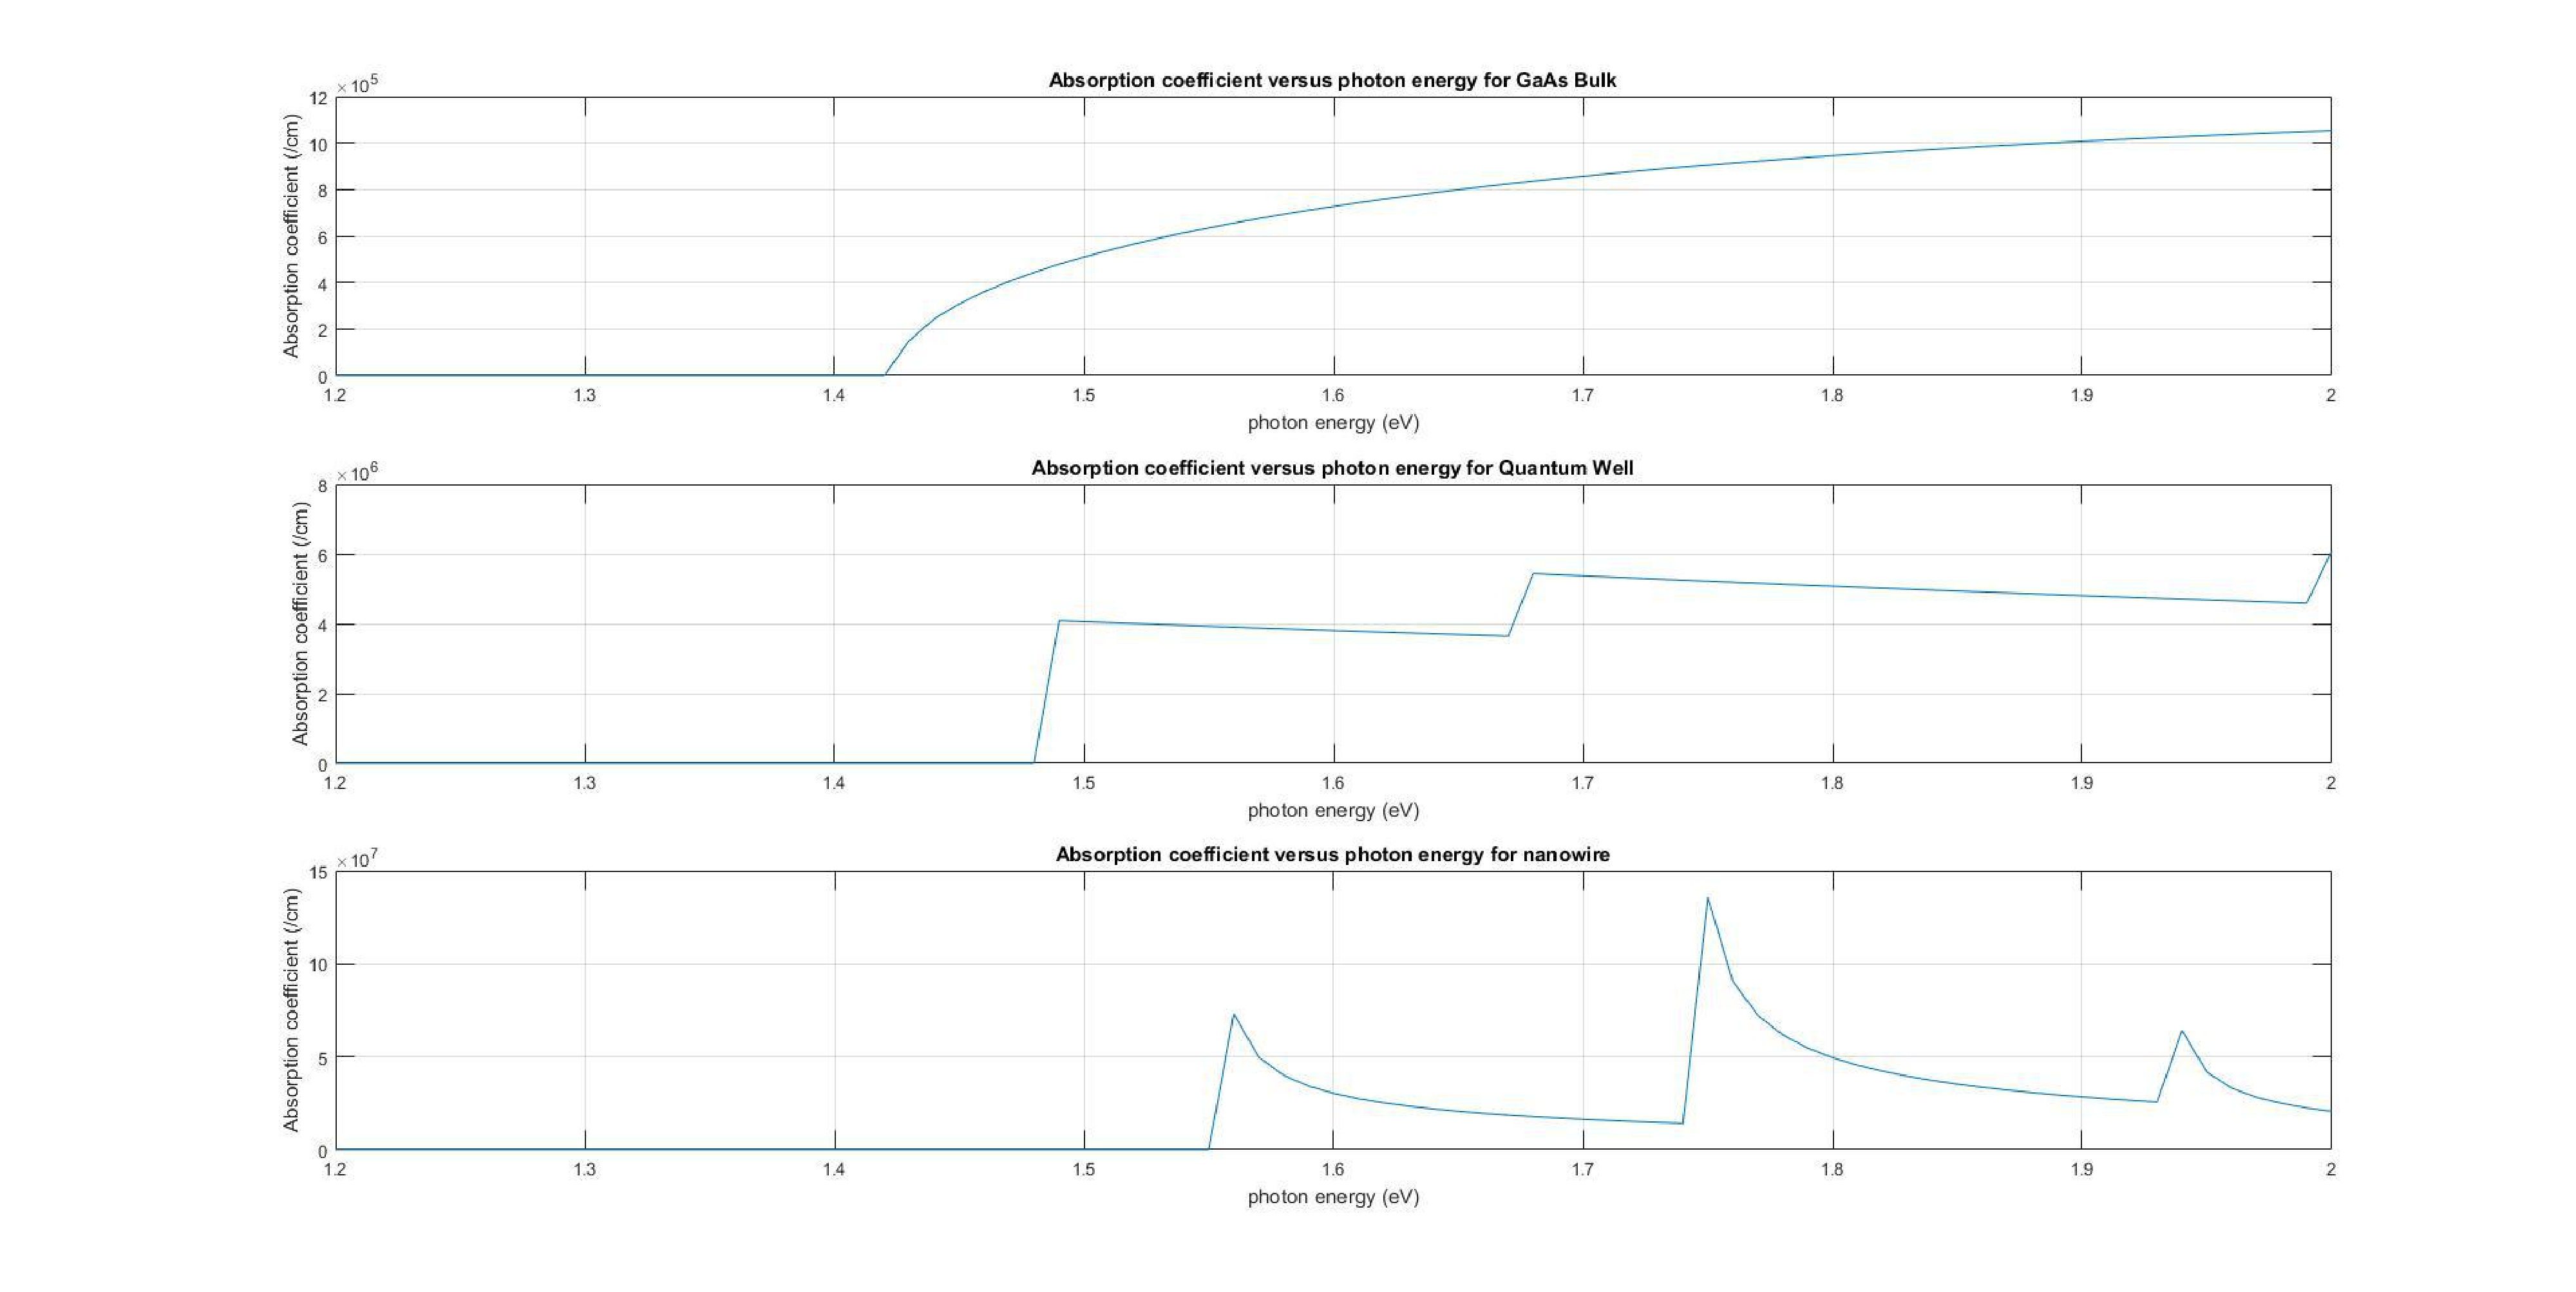
\includegraphics[width=\textwidth]{pictures/LT/absrate_split}
  \label{absrate_split}
\end{figure}

Then the overlay plot with multiple y axis as in Fig.~\ref{absrate_overlay} and
the different scales indicating the enhancement factor for 1D is 35(need to be
verified) compared to 3D.

\begin{figure}
  \caption{Absorption Coefficient versus Photon Energy for 1D 2D and 3D}
  \centering
  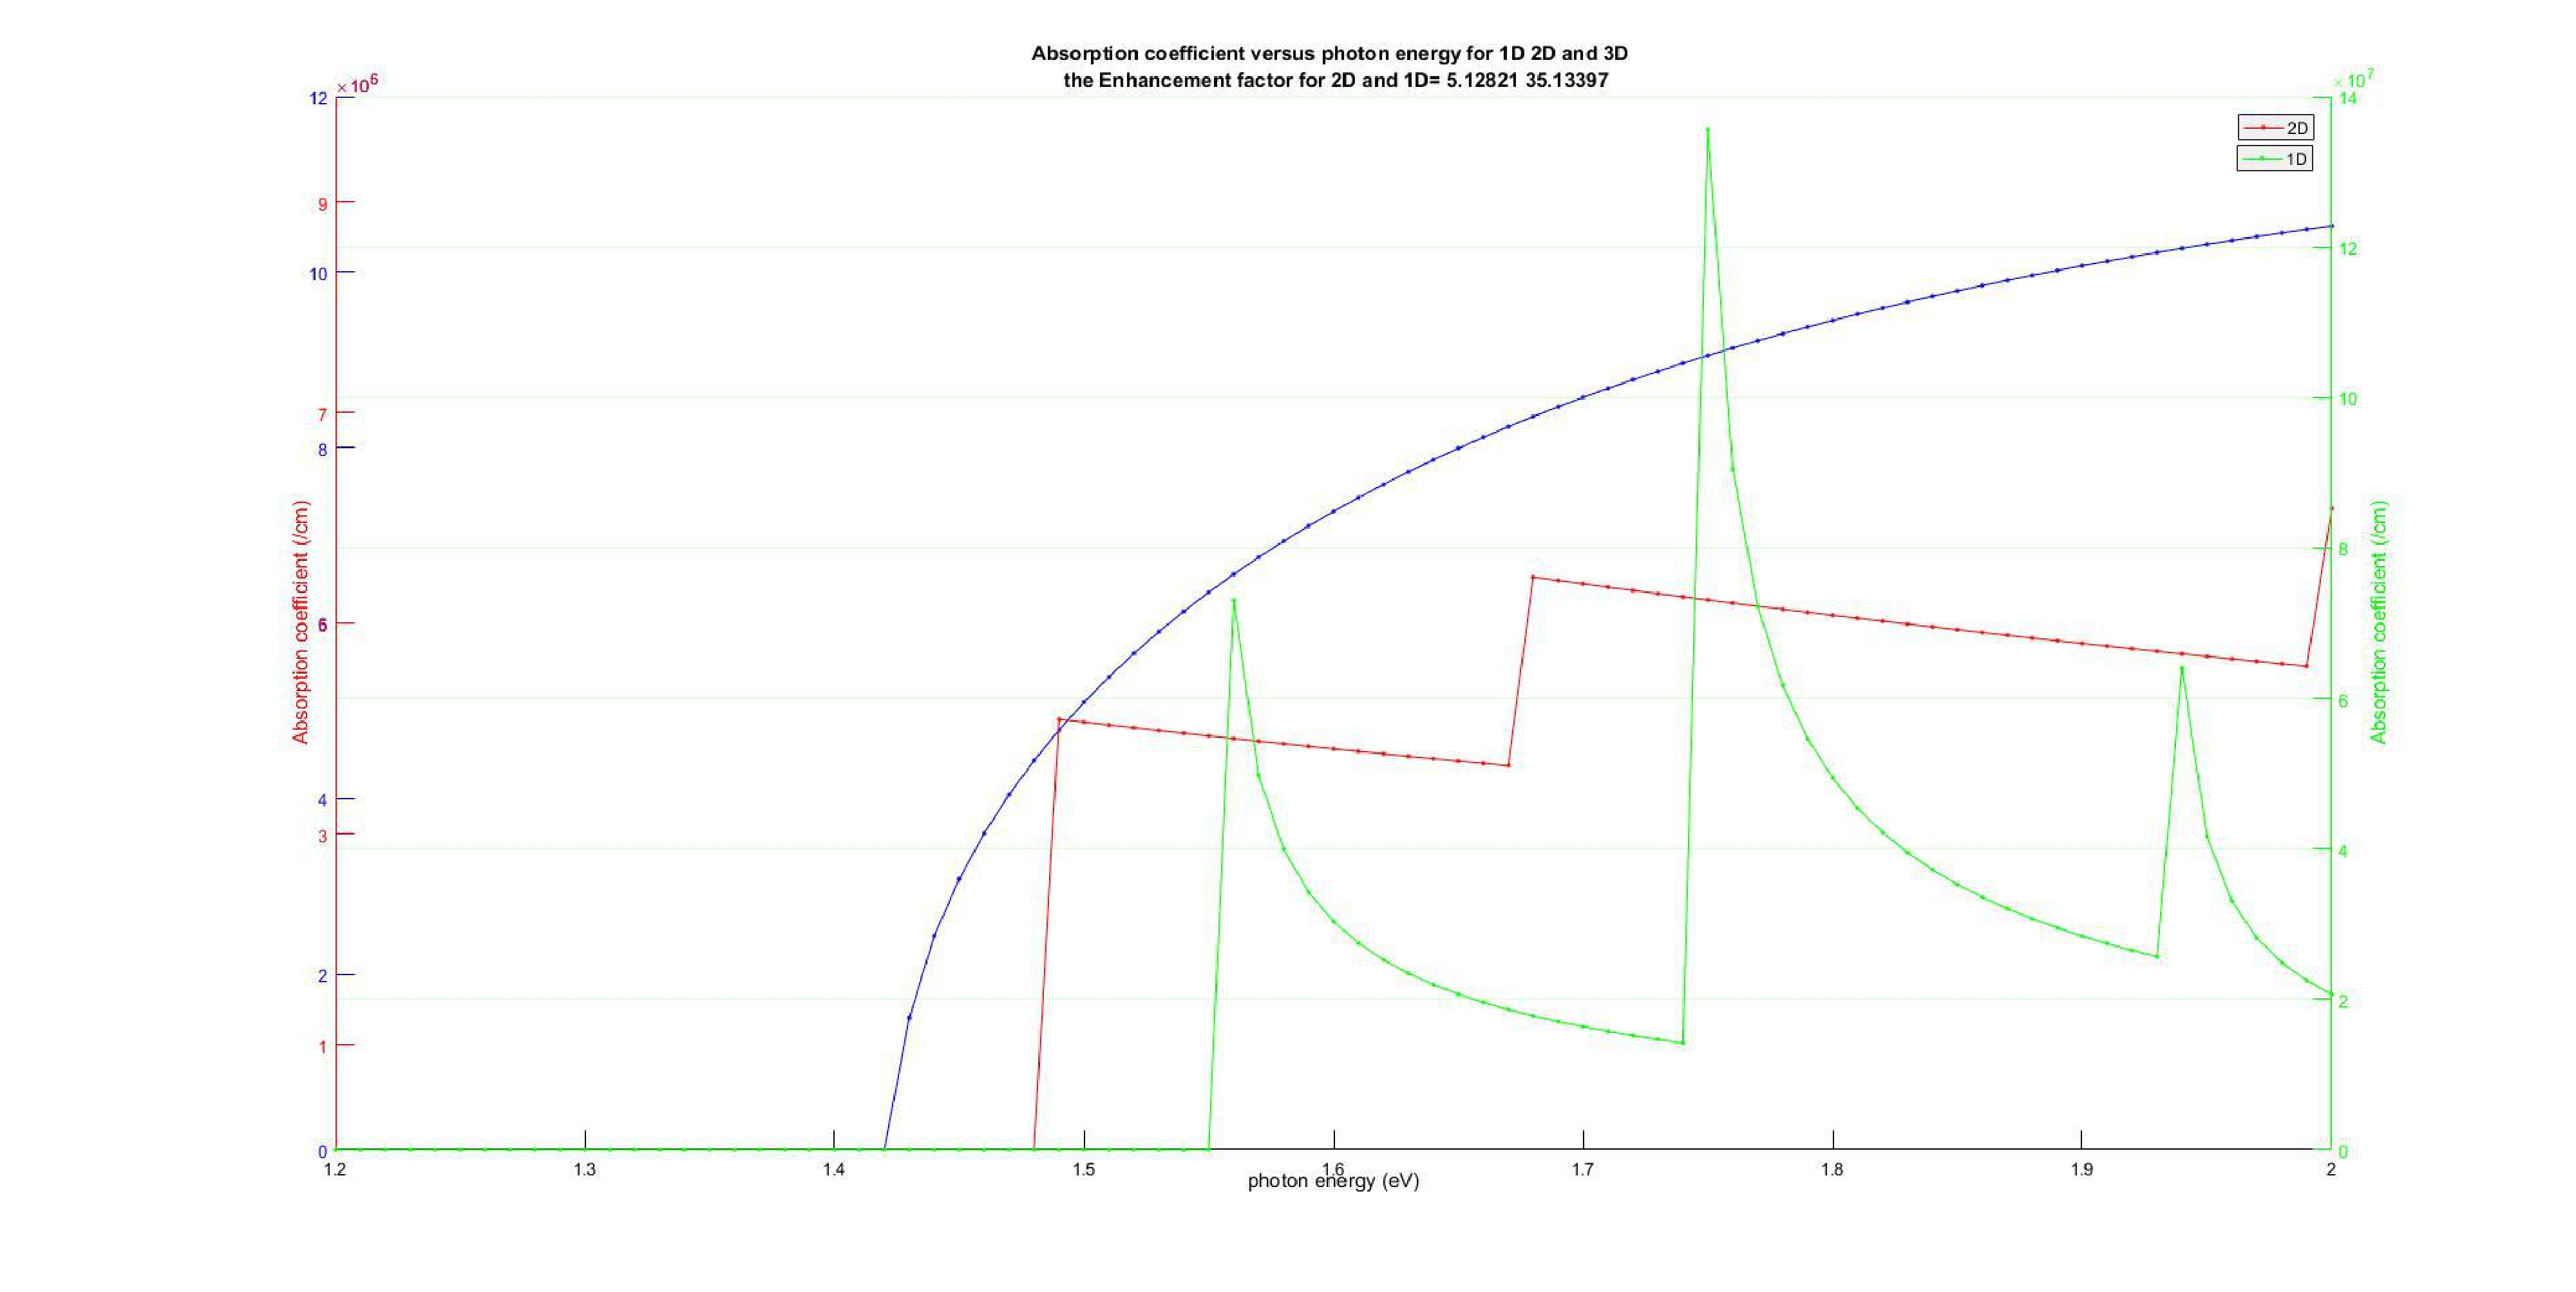
\includegraphics[width=\textwidth]{pictures/LT/absrate_overlay}
  \label{absrate_overlay}
\end{figure}

\subsection{Optical Gain}

Following the treatments of Appendix 3, we can derive the gain spectrum for 3D,
2D and 1D with consideration of occupation factor by calculating the Fermi
levels.

With decreasing dimensionality of the active region of an injection laser, the
density of states and gain spectra become narrower, which leads to a decrease
in the number of states to be filled to make the active region transparent
(zero population inversion and zero gain) and to achieve lasing (gain equal to
loss). Consequently, the transparency current (or inversion current, i.e., the
injection current at which the population inversion is zero) and the threshold
current (injection current at which the gain is equal to the loss and lasing
begins) decrease and their temperature dependences become weaker. The decrease
in the threshold current and increase in its temperature stability reflect one
fo the main areas of development and improvement of injection lasers. Owing to
the continuous nature of the carrier spectrum within the allowed subbands, the
use of QWs or QURs as active medium for optical transitions can only
quantitatively improve the parameters of devices based on them compared with
devices with a bulk active region. 

Among the advantages of QD lasers over the presently used QW lasers are their
narrower gain spectra, much lower threshold currents, and ultrahigh temperature
stability, as well as the wider possibilities for controlling their lasing
wavelength.

\begin{eqnarray}
\begin{aligned}
  & g_{3D}(\xi)=\frac{\sqrt{2}e^2{m_r^\ast}^{3/2}{p_{cv}^2}}{3{\pi}n_r\epsilon_0{m_0}^2C{\hbar^2}\xi}{\sqrt{(\xi-\xi_g)}}(f_n(\xi_2)-f_p(\xi_1)),
\\
& g_{2D}(\xi)=\frac{e^2{m_r^\ast}{p_{cv}^2}}{3{n_r}\epsilon_0{m_0}^2C{\hbar}L_z\xi}(f_n(\xi_2)-f_p(\xi_1)),
\\
& g_{1D}(\xi)=\frac{e^2{m_r^\ast}^{3/2}{p_{cv}^2}}{3{n_r}\epsilon_0{m_0}^2C\xi{L_x}{L_y}}\frac{1}{\sqrt{(\xi-\xi_g)}}(f_n(\xi_2)-f_p(\xi_1)),
\end{aligned}
\label{eq:five}
\end{eqnarray}

Now we can plot the gain spectrum respect to photon energy for 3D, 2D and 1D in
the figure below. As we can see, the gain spectrums follow the unique shapes of
density of states. The fourth figure is the maximum gain versus electron
carrier concentration varing from $3\times10^{18} (cm^{-3})$ to
$3\times10^{19}(cm^{-3})$. Using parameters $N_{tr} = 2\times10^{18} cm^{-3}$,
$N_{s} = 4\times10^{18} cm^{-3}$, and $g_0 = 6.11\times10^{5} cm^{-1}$, we fit
the curve in Fig.~\ref{gainspectrum} to build a logarithmic gain model of the
form for 3D case:

\begin{equation}
  g(N) = g_0\ln\left(\frac{N+N_s}{N_{tr}+ N_s}\right)
\end{equation}

where $N_s$ is a shift to force the natural logrithm to be finite at $N = 0$
such that the gain equals the umpumped absorption due to the band-to-band
transitions, $N_{tr}$ is the transparency carrier density, and $g_0$ is the
gain coefficient. $N_{tr}$ and $g_0$ will be different for different
dimensionality.

\begin{figure}
  \caption{Gain Coefficient versus Photon Energy for 1D 2D and 3D}
  \centering
  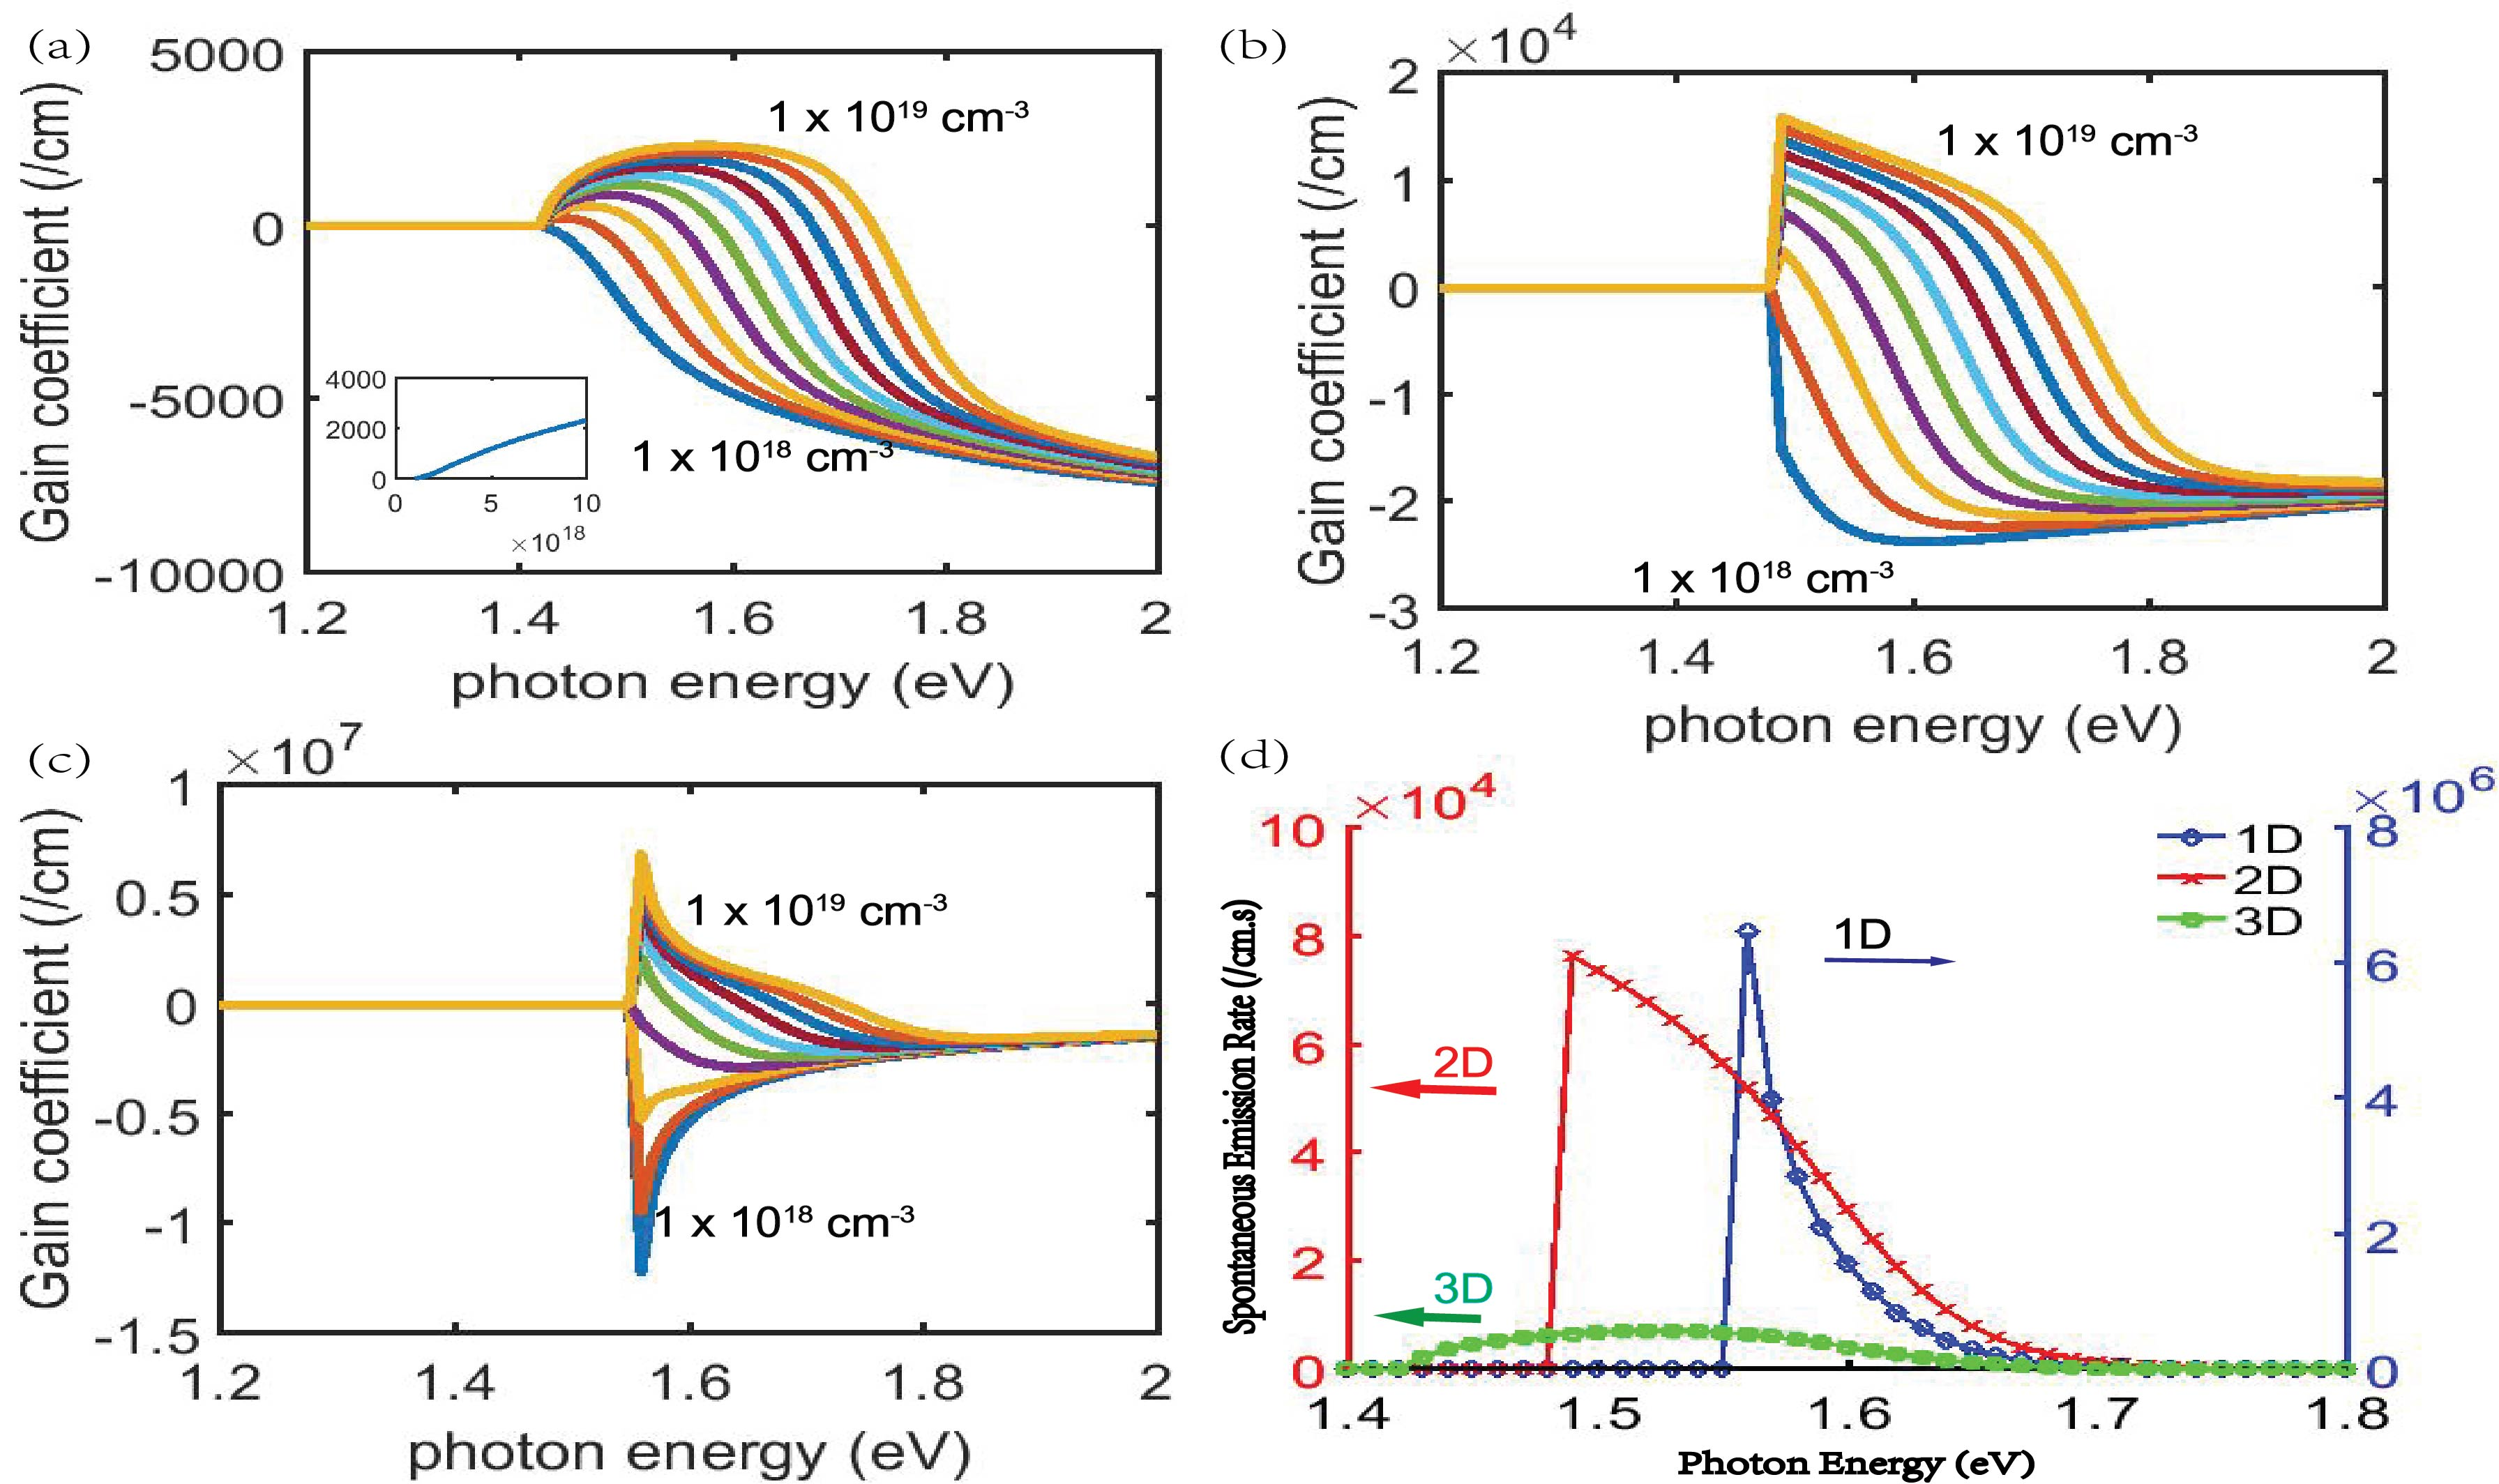
\includegraphics[width=\textwidth]{pictures/LT/gainspectrum}
  \label{gainspectrum}
\end{figure}

\begin{figure}
  \caption{Gain Model Fitting}
  \centering
  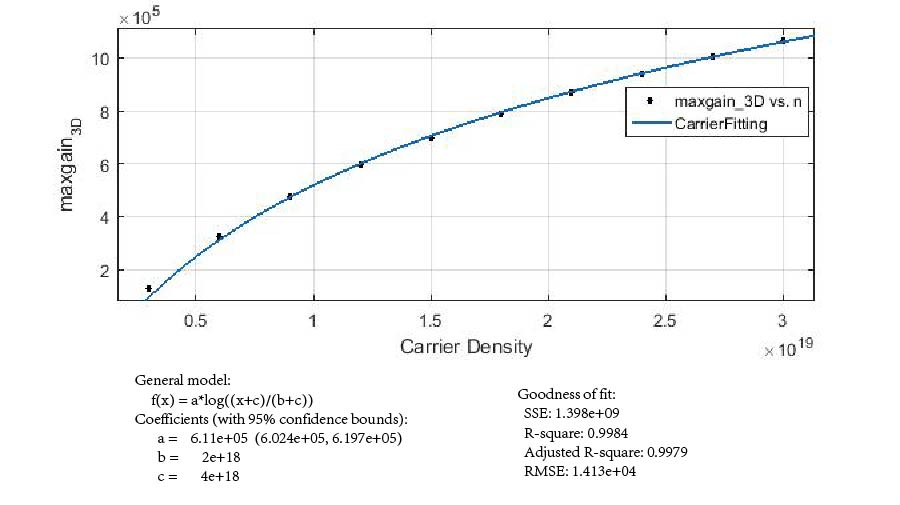
\includegraphics[width=\textwidth]{pictures/LT/gainModelFit_Anoted}
  \label{gainModelFit_Anoted}
\end{figure}

After fitting the curve in Fig.~\ref{gainModelFit_Anoted}, we can calculate the
threshold carrier density is $N_{th} = 4.533\times10^{18} cm^{-3}$. Then
plotting the spontaneous emission rate with respect to the threshold carrier
density $N_{th}$ for 3D, 2D and 1D as following: 

\begin{eqnarray}
\begin{aligned}
& r_{3D}^{\mathrm{spon}}(\xi)=\frac{n_re^2\xi{p_{cv}^2}}{{\pi}\epsilon_0{m_0}^2C^3{\hbar^2}}\frac{{m_r^\ast}^{3/2}}{2\pi^2\hbar^3}{\sqrt{(\xi-\xi_g)}}f_n(\xi_2)(1-f_p(\xi_1)),
\\
& r_{2D}^{\mathrm{spon}}(\xi)=\frac{n_re^2\xi{p_{cv}^2}}{{\pi}\epsilon_0{m_0}^2C^3{\hbar^2}}\frac{{m_r^\ast}}{\pi\hbar^2L_z}f_n(\xi_2)(1-f_p(\xi_1)),
\\
& r_{1D}^{\mathrm{spon}}(\xi)=\frac{n_re^2\xi{p_{cv}^2}}{{\pi}\epsilon_0{m_0}^2C^3{\hbar^2}}\frac{{m_r^\ast}^{3/2}}{\pi\hbar{m_e^\ast}L_xL_y}\frac{1}{\sqrt{(\xi-\xi_g)}}f_n(\xi_2)(1-f_p(\xi_1)),
\end{aligned}
\label{eq:six}
\end{eqnarray}

\begin{figure}
  \caption{Spontaneous Emission Rate versus Photon Energy for 1D 2D and 3D}
  \centering
  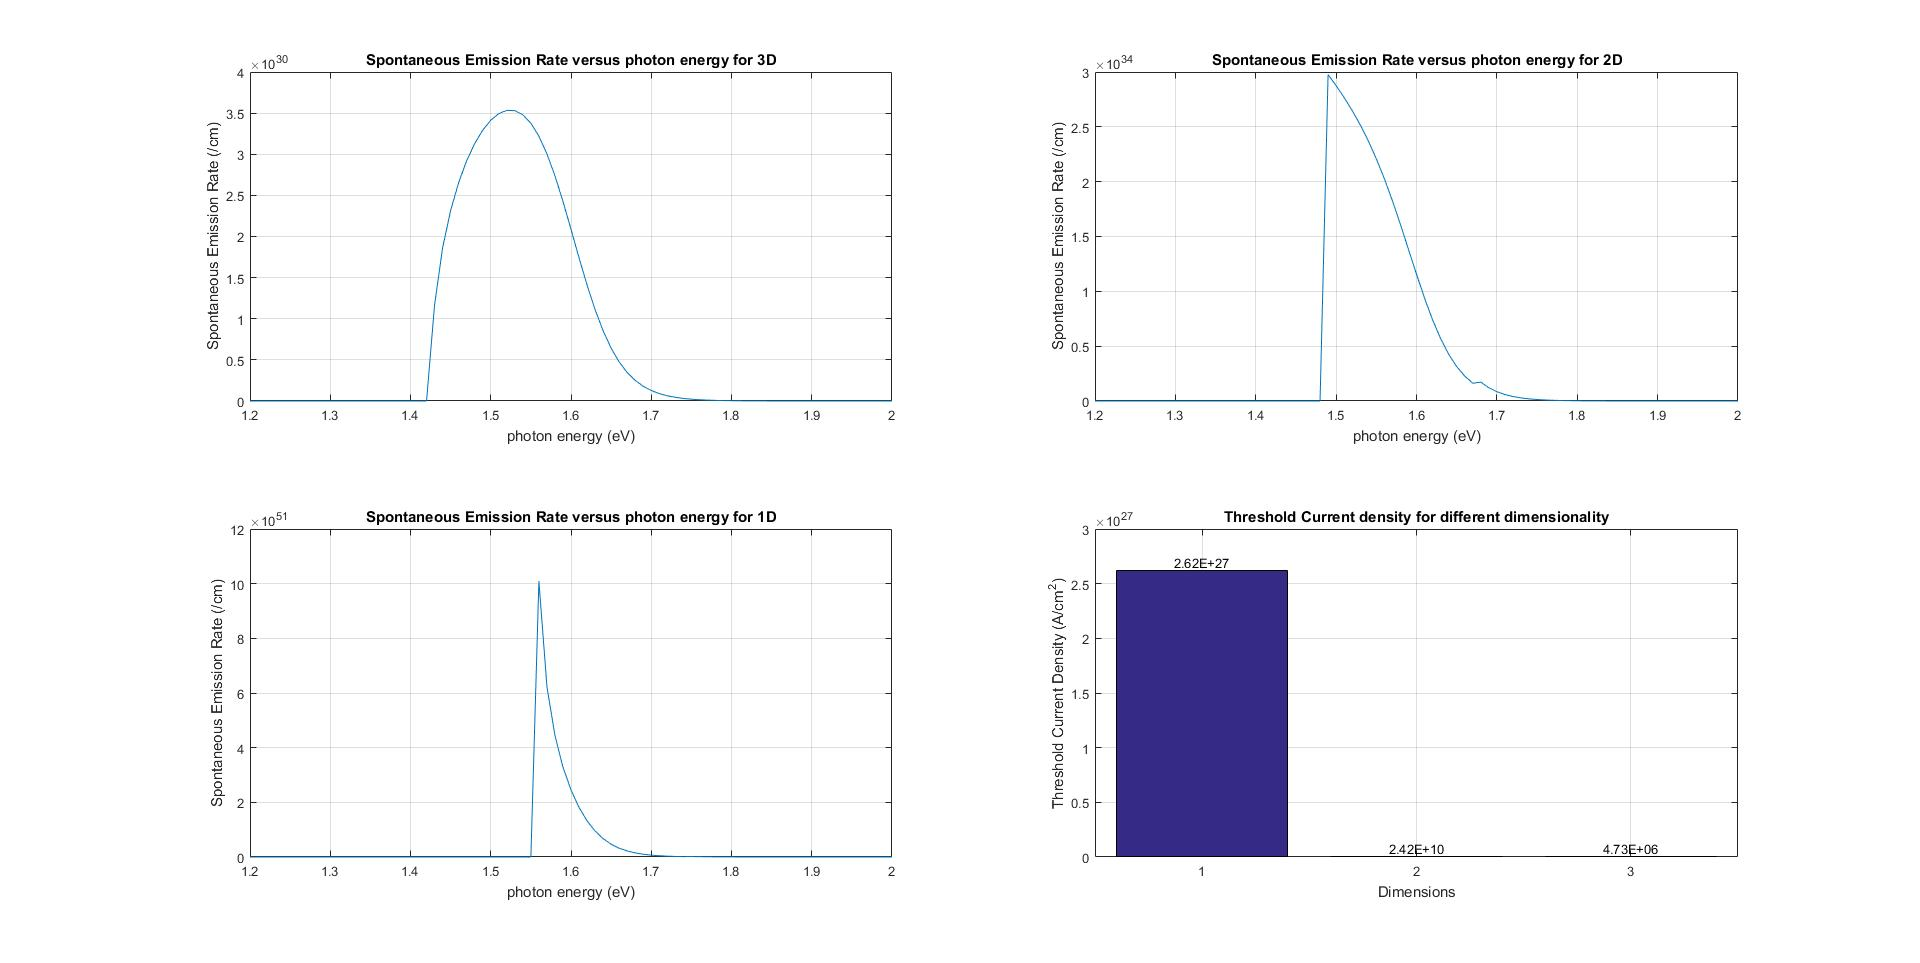
\includegraphics[width=\textwidth]{pictures/LT/sponrate}
  \label{sponrate}
\end{figure}

Integraing over all the photn energy spectrum, we have $R_{sp} =
\int_{\xi}r_{sp}d{\xi}$ for different dimensionality, then the threshold
current density can be simply caluclated as: $J_{th}= qdR_{sp}|_{N_{th}}$ and
plotted in the fourth part of Fig.~\ref{sponrate}. The threshold current for 3D
is $2.62\times10^{27} (A/cm^2)$, 2D is $2.42\times10^{10} (A/cm^2)$, and 1D
case is $4.73\times10^{6} (A/cm^2)$. The threshold current density needed for
lower-dimensional structure is greatly reduced.

Next, we can do dynamic analysis of laser modal and replace the threshold
current density to threshold pumping power. And verify the result with the
experimental data.

\subsection{Feedback and Laser Threshold}
\section{Types of semiconductor Lasers} \label{corrections}
\subsection{Fabry-Perot Semiconductor Lasers}

The Fabry-Perot(FP) laser is conceptually just an LED with a pair of end
mirrors or facets. The mirrors are needed to create the right conditions for
lasing to occur. The lasing medium can only amplify (undergo stimulated
emission) over a fairly narrow range because of the characteristics of the
material it is made from . A typical gain curve is illustrated on the
left-hand. 

\subsection{Grating-Based semiconductor Lasers}
\subsection{Vertical-Cavity Surface-Emitting Lasers}

As seen, light in the VCSEL propagates vertically with DBR mirrors as the
nature of the manufacturing process, the entire round-trip of the VCSEL is much
shorter than that of with the edge-emitting lasers. It leads to high
reflectivity ( around 99.9$\%$) of DBR mirrors, in which the large number of
layers are required.

One of features related to the VCSELs is the longitudianl modal stability due
to its short cavity length (around order of the wavelength). A

\subsection{Grating Surface-Emitting Lasers}
\section{Characteristics of Semiconductor Lasers} \label{corrections}

In order to understand their operation, it is necessary to know some basic
performance parameters or important features of semiconductor lasers.

\section{Basic Requrement for Design of Semiconductor Lasers} \label{corrections}
\subsection{Spectral width and Linewidth}

FP semiconductor lasers produce a range of wavelengths. This range of
wavelengths is called the "spectral width" of the laser. Typically there will
be around 8 "modes" and the spectral width. In order to determin exactly the
spectral shape, spectral width is usually quoted as the FWHM (Full Width Half
Maximun) Instead of producing a continuous range of wavelengths over their
spectral width. Semiconductor lasers produce a series of "lines" at a number of
discrete wavelengths. Lines themselves vary in width (in different types of
lasers) very significantly. The linewidth is inversely proportional to the
coherence length of the laser.

\subsection{Operating Wavelength, Switching Time, and Modulation}
\section{Modeling of Semiconductor Lasers} \label{corrections}

From the general formulations through the rate equations ans wave equations
based on the

As we know, from different aspects of the same physics of the energy
conservation, there are two basic classical methods to model the operation of
semiconductor lasers. The first method, which will be summarized , applies the
concept of photo/electron particle exchange with the abtract optical parameters
and is suitable for the FP lasers. For the DBR/DFB lasers, due to strong
non-uniformities of index distribution. The interaction between electromagnetic
fields and electric particles has been considered, which . Indeed, those two
methods are wholly compatible with one anohter. In this project, because we
focus on the FP lasers as , we employ the first method: the standard rate
equation approach.

Three fundamental elements in the semiconductor lasers: semiconductor band
structure, current injection, and cavity. The former two are related to the
material and junction structure, and the later is related to the laser
structure. For semiconductor lasers, the key in the modeling is to deal with
the interaction between electromagnetic fields and gain medium. The basic
procedure of modeling of semiconductor lasers: Due to the complexity of the
rate equation and coupling between carrier and photon density, the coupling
rate equations are further solved by numerical methods such as the
standing-wave approach (in frequency domain) and the traveling-wave approach
(in time domain). The stading-wave approach is based on the assumption that the
temporal and the spatial dependence of field distributions of the cavity odes
are separable. As such, the dynamics is considered in the modal amplitudes.
Consequently, the standing-wave apporach is valid only when the photon lifetime
is much shorter than the characteristic time of the laser dynamics. The
traveling-wave approach, on the other hand, makes no assumptions about the
cavity modes. Rather, it solves the time-dependent coupled=wave equations for
the forward and the backward traveling waves directly and tehrefore is valid
even the laser cavity has relatively small Q-factor and/or the characteristic
time of the laser dynamics is very short. Another advantage of the
traveling-wave model is that it can be readily applied to laser diodes operated
with multiple cavity modes, for which the stading-wave model may have
difficulty in finding the complex roots corresponding to each mode.
\section{Laser Rate Equations} \label{corrections} 


We start with the governing equations of carrier density and photon density in
the active region which is governed by a dynamic process.

\begin{eqnarray}
\begin{aligned}
  & \frac{dN}{dt} = \frac{\eta_{i}I}{qV} - \frac{N}{\tau} - R_{st},
  \\
  & \frac{dN_p}{dt} = {\Gamma}v_g{g}N_p + \Gamma\beta_{sp}R_{sp} - \frac{N_p}{\tau_p},
\end{aligned}
\label{eq:eight}
\end{eqnarray}

where $\beta_{sp}$ is the spontaneous emission factor, defined as the
percentage of the total spontaneous emission coupled into the lasing mode. And it is
just the reciprocal of the number of available optical modes in the bandwidth of
the spontaneous emission for uniform coupling to all modes. The g is Incremental gain
per unit length.

The first term of equation 1 is the rate of injected electrons $G_{gen} =
{\Gamma_{i}I}/{qV}$, ${\Gamma_{i}I}/{q}$ is the number of electrons per
second being injected into the active region, where V is the volume of the
active region. The rest terms are the rate of recombining of electrons per unit
volume in the active region. There are several mechanisms should be considered,
including a spontaneous recombination rate, $R_{sp}$, a nonradiative
recombination rate, $R_{nr}$, a carrier leakage rate, $R_l$ and a net
stimulated recombination, $R_{st}$, including both stimulated absorption and
emission. Which looks like:

\begin{equation}
  R_{rec} = R_{sp} + R_{nr} + R_{l} + R_{st}
\end{equation}

The above equation used input current intensity, $I$, for electrically injected
lasing situation, however, if optical pump used as the lasing source, then we
need to rewrite the governing equations.

\begin{eqnarray}
\begin{aligned}
  & \frac{dN}{dt} = \frac{\eta_{i}P}{qV} - \frac{N}{\tau} - R_{st},
  \\
  & \frac{dN_p}{dt} = {\Gamma}v_g{g}N_p + \Gamma\beta_{sp}R_{sp} - \frac{N_p}{\tau_p},
\end{aligned}
\label{eq:eight}
\end{eqnarray}

$P$ is the optical pump used for exciting nano-cavity laser emission and is
time-dependent of the form $P_{p}sech^2(\frac{1.76t}{\delta{t}})$, where $P_p$ is the peak power amplitude, and $\delta{t}$ is the time pulse width.


The cavity loss can be characterized by a photon decay constant or lifetime,
$\tau_p$, and the gain necessary to overcome losses, and thus reach threshold.
By assuming steady-state conditions (\ie $dN_p/dt = 0$), and solving for this
steady-state or threshold gain, $g_{th}$, where the generation term equals the
recombination term for photons. We assume only a small fraction of the
spontaneous emission is coupled into the mode (\ie $\beta_{sp}$ is quite
small), then the second term can be neglected, and we have the solution:

\begin{equation}
  \Gamma{g_{th}} = \frac{1}{v_g\tau_p} = <\alpha_i> + \alpha_m
\end{equation}

The product, $\Gamma{g_{th}}$, is referred to as the threshold modal gain
because it now represents the net gain required for the mode as a whole, and it
is the mode as a whole that experiences the cavity loss. $<\alpha_i>$ is the
average internal loss, and $\alpha_m$ is the mirror loss if we considered an
in-plane wave laser.

\begin{equation}
  R_{rec} = R_{sp} + R_{nr} + R_{l} + R_{st}
\end{equation}

The first three terms on the right refer to the natural or unstimulated carrier
decay processes. The fourth one, $R_{st}$, require the presence of photon.


Then, recognizing that $(R_{sp} + R_{nr} + R_{l}) =AN + BN^2 +CN^3$ depends
monotonically on $N$, we observe from eq 2.34 that above threshold $(R_{sp} +
R_{nr} + R_{l})$ will also clamp at its threshold value, given by Eq 2.35. Thus,
we can substitute Eq 2.35 into the carrier rate equation, eq 2.16 to obtain a
new above threshold carrier rate equations,

\begin{equation}
  \frac{dN}{dt} = \eta_i \frac{(I - I_{th})}{qV} - v_{g}gN_p,~~~   (I > I_{th})
\end{equation}

We also calculate a steady-state photon density above threshold where $g = g_{th}$,

\begin{equation}
  N_p = \frac{\eta_i (I - I_{th})}{qv_{g}g{th}V}~~~   (steady~ state)
\end{equation}

To obtain the power out, we first construct the stored optical energy in the
cavity, $E_{os}$, by multiplying the photon density, $N_p$, by the energy per
photon, $hv$, and the cavity volume, $V_p$. That is $E_{os} = N_phvV_p$. Then,
we multiply this by the erngy loss rate through the mirrors, $v_g\alpha_m =
\frac{1}{\tau_m}$, to get the optical power output from the mirrors,

\begin{equation}
  P_0 = v_g\alpha_{m}N_phvV_p
\end{equation}

Substituting from , and using $\Gamma = V/V_p$,

\begin{equation}
  P_0 = \eta_i(\frac{\alpha_m}{<\alpha_i> + \alpha_m})\frac{hv}{q}(I - I{th}),~~~(I > I_{th})
\end{equation}


We can get the threshold carrier density

\begin{equation}
  N_{th} = N_{tr}e^{g_{th}/g_{0}N} = N_{tr}e^{(<\alpha_i> + \alpha_m)/\Gamma{g_{0}}N}
\end{equation}

Using the polynomial fit for the recombination rates, and recognizing that for
the best laser material the recombination at threshold is dominated by
spontaneous recombination, we have, $I_{th}\cong B{N_{th}}^2qV/\eta_i$, Thus

\begin{equation}
  I_{th} {\cong} \frac{qVB{N_{tr}}^2}{\eta_i}e^{(<\alpha_i> + \alpha_m)/\Gamma{g_0}N}
\end{equation}

where for most $\uppercase\expandafter{\romannumeral3} -
\uppercase\expandafter{\romannumeral5}$ materials the bimolecular recombination
coefficient, $B \sim 10^{-10} cm^3/s$.

Reduce the transparency value and increase the differential gain of the active
materials.

It is desirable to reduce the cavity loss $(<\alpha_i> + \alpha_m)$ and volume,
$V$, in order to retaining a reasonably large confinement factor, $\Gamma$.

\section{Wave Model of Semiconductor Lasers} \label{corrections}

\section{Linewidth Enhancement Factor} \label{corrections}

Electrons and holes frequently interact with other carriers and with phonons,
thereby changing their energy within the sub-band. Such intra-band scatter
events happen about every 0.1 ps, much more often than band-to-band
recombination events. Thus, scattering leads to an uncertainty of the electron
energy, which can be accounted for by introducing a symmetrical linewidth
broadening funtion L into the gain formula.  This convolution integral means
that gain at the photon energy can now receive contributions from electron
transitions with, weighted by 

In fact, positive gain is now possible even for photon energies slightly below
the bandgap. Cauchy himself exploited such a density function in 1827, with
infinitesimal scale parameter, in defining a Dirac delta function, while among
physicists, it is known as the Lorentzian line shape functionL with the
half-width. This function is based on the assumption that the occupation
probability of an electron state decays proportionally to exp(-t/). The Fourier
transformation of this exponential function into the nergy domain leads to .
Gamma is the average of the broadening in the conduction and inthe valence
band. The full linewidth 2gamma is related to the average intra-band scattering
time 

Which includes scattering events in the conduction band and valence band. For
each band, linewidth contributions from different scattering processes are
adding up.

\section{Implementations} \label{corrections}
\subsection{Optical Modes}
\subsection{Steady State Analysis}
\subsection{Dynamic State Analysis}

\section{Simulation Results} \label{corrections}
\subsection{Input Parameters}
\subsection{Optical Modes}
\subsection{Steady State Analysis}
\subsection{Dynamic State Analysis}
